%%%%%%%%%%%%%%%%%%%%%%%%%%%%%%%%%%%%%%%%%%%%%%%%%%%%%%%%%%%
% --------------------------------------------------------
% Rho
% LaTeX Template
% Version 2.1.1 (01/09/2024)
%
% Authors: 
% Guillermo Jimenez (memo.notess1@gmail.com)
% Eduardo Gracidas (eduardo.gracidas29@gmail.com)
% 
% License:
% Creative Commons CC BY 4.0
% --------------------------------------------------------
%%%%%%%%%%%%%%%%%%%%%%%%%%%%%%%%%%%%%%%%%%%%%%%%%%%%%%%%%%%

\documentclass[9pt,letterpaper,onecolumn]{rho-class/rho}
%\usepackage[english]{babel}

%% Spanish babel recomendation
\usepackage[spanish,es-nodecimaldot,es-noindentfirst]{babel}

\setbool{rho-abstract}{true} % Set false to hide the abstract
\setbool{corres-info}{true} % Set false to hide the corresponding author section

%----------------------------------------------------------
% TITLE
%----------------------------------------------------------

%\journalname{Example Template}
\title{DevGraph: Simulación de red social}

%----------------------------------------------------------
% AUTHORS AND AFFILIATIONS
%----------------------------------------------------------

\author[$\dagger$]{Franco Aguilar}
\author[$\dagger$]{Iván Mansilla}
\author[$\dagger$]{Diego Sanhueza}
\author[$\dagger$]{Duvan Figueroa}
\author[$\dagger$]{Miguel Maripillan}

%----------------------------------------------------------

%\affil[1]{Affiliation of author one}
%\affil[2]{Affiliation of author two}
%\affil[3]{Affiliation of author three}
\affil[$\dagger$]{Universidad de Magallanes}

%----------------------------------------------------------
% DATES
%----------------------------------------------------------

\dates{Informe fue compilado el día \today}

%----------------------------------------------------------
% FOOTER INFORMATION
%----------------------------------------------------------

%\leadauthor{Author last name et al.}
%\footinfo{Creative Commons CC BY 4.0}
\smalltitle{Estructuras de datos}
%\institution{Universidad de Magallanes}
\theday{\today} %\today

%----------------------------------------------------------
% ARTICLE INFORMATION
%----------------------------------------------------------

%\corres{Provide the corresponding author information and publisher here.}
%\email{example@organization.com.}
%\doi{\url{https://www.doi.org/exampledoi/XXXXXXXXXX}}

%\received{March 20, 2024}
%\revised{April 16, 2024}
%\accepted{April 20, 2024}
%\published{May 21, 2024}

%\license{Rho LaTeX Class \ccLogo\ This document is licensed under Creative Commons CC BY 4.0.}

%----------------------------------------------------------
% ABSTRACT
%----------------------------------------------------------

\begin{abstract}
    DevGraph es una simulación de una red social, enfocada en la creación de usuarios, la conexión entre ellos, la visualización y creación de publicaciones, y la posible sugerencia de amistades y publicaciones. Para esto se utilizaron grafos, listas enlazadas, tablas hash, colas de prioridad, algoritmos de similaridad, etc.
\end{abstract}

%----------------------------------------------------------

\keywords{C, Grafos, Red Social, Simulación, Estructuras de Datos}

%----------------------------------------------------------

\begin{document}
	
    \maketitle
    \thispagestyle{firststyle}
    \tableofcontents
    %\linenumbers


%----------------------------------------------------------
% INTRODUCCION
%----------------------------------------------------------
\newpage
\section{Introducción}
	\rhostart{U}na red social es una aplicación diseñada para conectar a las personas y permitirles compartir información a través de publicaciones. Estas plataformas toman en cuenta los intereses y preferencias de los usuarios, ayudándoles a formar comunidades, establecer amistades y ver contenido relevante basado en sus gustos o conexiones.

DevGraph es una simulación de una red social que se enfoca en la creación de usuarios, la conexión entre ellos, la visualización y creación de publicaciones, y la posibilidad de compartirlas. Además, incluye algoritmos que simulan sugerencias de nuevos amigos y publicaciones relevantes para los usuarios.

Para su implementación en C, se utilizaron algoritmos y estructuras de datos para simular DevGraph como:

\begin{itemize}

\item \textbf{Estructuras de datos:}
\begin{itemize}
\item \textbf{Grafos:} En representación de las conexiones entre usuarios, donde cada persona corresponde a un vértice y cada conexión una arista en un grafo dirigido.
\item \textbf{Tablas Hash:} Para una busqueda eficiente de datos en la red social.
\item \textbf{Colas de prioridad (Heap):} Para crearon recomendaciones de usuarios y publicaciones en base a nuestros intereses o amigos.
\item \textbf{Listas enlazadas:} Para manejar publicaciones como listas enlazadas de nodos.
\end{itemize}
\item \textbf{Algoritmos:}
\begin{itemize}
\item \textbf{Algoritmo de caminos cortos (Dijkstra):} Para calcular la distancia de un nodo a otro en un grafo y de ésta manera encontrar usuarios cercanos en la red.
\item \textbf{Similaridad de Jaccard:} la cual mide el peso del enlace en base a los intereses comunes entre dos usuarios.
\end{itemize}
\item \textbf{Funcionalidades adicionales:}
\begin{itemize}
\item Generación de usuarios aleatorios.
\item Almacenamiento y recuperación de datos.
\item Perfíl psicológico.
\end{itemize}

\end{itemize}

%----------------------------------------------------------
% OBJETIVOS
%----------------------------------------------------------
\section{Objetivo Principal}
	\rhostart{E}l objetivo principal del proyecto es crear una simulación de una red social eficiente y rápida, combinando armónicamente los distintos tipos de estructuras de datos vistos durante el curso de Estructuras de Datos (grafos, listas, hash tables, colas de prioridad, etc.).

\subsection{Objetivos secundarios}
\begin{itemize}
	\item Implementar algoritmos de búsqueda eficientes, priorizando el tiempo de respuesta.
	\item Implementar buenas prácticas de codificación.
	\item Reforzar habilidades de trabajo en equipo y coordinación de tareas entre pares.
	\item Reforzar habilidades de investigación y análisis de datos.
\end{itemize}

\newpage
%----------------------------------------------------------
% PLANTEAMIENTO
%----------------------------------------------------------
\section{Planteamiento del desarrollo del proyecto}


\subsection{Usuarios y Posts}

\rhostart{L}os usuarios y los posts resultan el elemento más importante del programa, pues prácticamente todo el funcionamiento se centra en ellos, por lo que era fundamental que estos estuvieran constituidos de la forma más correcta y eficiente posible. Ambos elementos de forma automática se optó por crearlos como estructuras, que contengan la información pertinente a cada uno, estructuras que se definieron como tipo de dato con typedef, para así en el código tener una mejor comprensión y orden.

\subsubsection{Usuarios}
Para definir la información de los usuarios que estarían en su estructura se observaron y analizaron los elementos de distintas redes sociales, de los cuales se concluyó que en su mayoría poseen:
\begin{itemize}
	\item Nombre
	\item Contraseña
	\item Usuario
	\item Lista de seguidos
	\item Lista de seguidores
	\item Posts
\end{itemize}

Por lo que, estos elementos fueron considerados. Además de esto, a medida de que el proyecto fue avanzando y las necesidades evolucionando, se fueron agregando más variables a esta estructura, tal y como sus intereses.

\vspace{0.5cm}

De la estructura planteada anteriormente resalta la palabra “Lista”. Se sabe que las redes sociales en sí las conexiones entre usuarios funcionan como un grafo, en donde un usuario puede tener enlaces con múltiples personas; por lo tanto, estos enlaces de dicho grafo en este caso serían representados por la lista de seguidos y seguidores. Entonces, la estructura de un usuario pasaría a ser el nodo de un gráfico, y las listas, las listas de adyacencia de este. Con esto claro, se unificaron los usuarios con la estructura de datos de los grafos, que estaba siendo trabajada en paralelo. 

\vspace{0.5cm}

Sin embargo, este enfoque trajo como consecuencia un problema importante: la búsqueda. El tener que recorrer el grafo en el peor de los casos en orden O(n) para encontrar un único usuario resulta sumamente ineficiente y costoso, sobre todo si hay un gran flujo de datos. Por lo tanto, para resolver esto se pensó en la estructura de datos que tiene un orden de búsqueda O(1): las tablas hash. Entonces, además de los usuarios encontrarse dentro del grafo, a estos se les ve asignado un ID según su nombre de usuario, ID que representa su posición en una tabla hash global en donde están representados todos los usuarios de la red. Este agregado dio al programa la velocidad de búsqueda buscada eficientemente.

\subsubsection{Posts}
Los posts (o publicaciones) inmediatamente se asumieron como una lista enlazada, en donde la inserción es al principio de ella para mantener un orden de “más reciente a más antiguo”. Al igual que los usuarios, se investigaron las características de otras redes sociales, de donde resaltó que los posts usualmente suelen tener:
\begin{itemize}
	\item Fecha
	\item Contenido del post
\end{itemize}
	Por lo que estos elementos fueron añadidos a su estructura.

	Con esto hecho, fue lógico, que para que un post sea relacionado a un usuario en específico, que cada usuario tenga en su estructura su lista de posts propia

\subsection{Intereses y Similaridad}
	\rhostart{L}os algoritmos de similaridad son técnicas para verificar que tan iguales son dos conjuntos. En el caso de una red social, esto resulta una característica importante para los algoritmos de recomendación de usuarios y publicaciones, así manteniendo enganchado al usuario con contenido que realmente le interese.

	Una característica que fue en cierto sentido difícil de plantear fueron cómo representar los intereses de los usuarios de la forma más eficiente, y que sea fácil de obtener su similaridad con los intereses de otro. 
	Desde un principio se eligió trabajar con el \textbf{índice de Jaccard}, el cual básicamente habiendo dos conjuntos A y B, su similaridad estará dada por la intersección entre estos dividida por su unión. O sea:
    \begin{equation}
        \label{eq:jaccard}
        J(A,B) = \frac{|A \cap B|}{|A \cup B|}
    \end{equation}
    Esto es un cálculo matemático bastante fácil, el problema era cómo aplicarlo a un grafo y cómo representar los intereses de tal forma que coincidiera con esto.

    \vspace{0.5cm}
	
	Entonces, después de una investigación, se acordó utilizar para los intereses atributos binarios. O sea, que cada usuario tuviese una tabla en donde cada celda representa un interés en específico, almacenando un valor “0” si no tiene el interés o “1” si lo tiene. Este enfoque hizo que el índice de jaccard fuese sumamente fácil de calcular, pues es tan simple como sumar la cantidad de celdas en los que ambos tienen un “1” y dividirlo por la cantidad total de intereses presentes. 

    \begin{figure}[H]
        \centering
        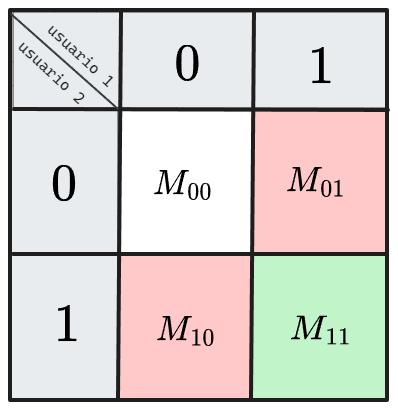
\includegraphics[width=0.3\textwidth]{figures/tablas_intereses.png}
        \caption{Tabla comparativa de intereses entre 2 usuarios}
        \label{fig:tablas_intereses}
    \end{figure}

    $M_{00}$ es el N° de intereses donde ambos tienen valor 0, $M_{10}$ N° de intereses donde el usuario 1 tiene valor 1 y el usuario 2 0, y así sucesivamente. Por lo tanto, la formula para calcular la similitud entre dos usuarios es:

    \begin{equation}
        \label{eq:jaccard}
        J(U1,U2) = \frac{M_{11}}{M_{01}+M_{10}+M_{11}}
    \end{equation}
	
	Sin embargo, esto de igual forma trajo de duda si se estaba ocupando la memoria eficientemente, ya que se estaría guardando la información de qué interés es cada celda repetidas veces. Por lo tanto, se creó una tabla global de intereses, el cual simplemente almacena qué interés corresponde a cada celda, así los usuarios únicamente almacenando en su tabla un puntero a dicha tabla y el valor que le corresponde.

%------------------------------------------
%------------------------------------------
\subsection{Grafos}
\rhostart{U}n grafo es una estructura de datos utilizada para modelar relaciones entre entidades. En este caso, se utilizaron para representar la red social, donde cada nodo, como se dijo anteriormente, representa un usuario. Los grafos se encuentran presentes como estructura de datos fundamental en practicamente todas las redes sociales, pues cada usuario tiene diversas conexiones salientes y entrantes con otros usuarios. Por lo que su implementación fue considerada desde un principio.

\vspace{0.5cm}

En un principio se tuvo la disyuntiva si para aplicar el grafo utilizar una matriz de adyacencia, o bien una lista de adyacencia, y de hecho lo que fue desarrollado en las primeras versiones del programa fue una matriz de adyacencia. Sin embargo, esto no era eficiente ni correspondiente, ya que presentaba una limitación en cuanto a la cantidad de usuarios como en la cantidad de conexiones que se podrían crear; además, los usuarios habían sido pensados que tuvieran una lista de seguidos y seguidores, que eran listas enlazadas simples. Por lo tanto, se deicidió utilizar listas de adyacencias, que permitían la representación de relaciones entre usuarios de manera más eficiente, y que se adaptaba bien a grafos dispersos.

\vspace{0.5cm}

La utilización de grafos con listas de adyacencia, como se dijo anteriormente, de todas formas trajo algunos problemas, tales como la búsqueda, que fue resuelta con tablas hash, recorrer el grafo, y la busqueda de caminos cortos.

\vspace{0.5cm}

Para recorrer el grafo en su totalidad, se decidió hacer que los usuarios no solo sean nodos de un grafo, sino que también nodos de una lista enlazada. O sea, que al crear un grafo, lo que se crea en realidad es una lista enlazada simple, en donde cada nodo es también un nodo de un grafo con diversas conexiones salientes y entrantes. 

\begin{figure}[H]
    \centering
    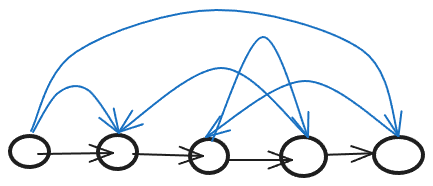
\includegraphics[width=0.3\textwidth]{figures/grafo.png}
    \caption{Representación del grafo de usuarios}
\end{figure}

Por otro lado, para la búsqueda de caminos cortos, se decidió utilizar el algoritmo de Dijkstra, que se utiliza para encontrar el menor camino entre dos nodos en un grafo. Se tuvo la duda si utilizar otros algoritmos como por ejemplo el algoritmo de BFS, pero finalmente fue descartado por una mayor simplicidad.

\subsection{Generación de usuarios aleatorios}
\rhostart{L}a generación de usuarios aleatorios es un proceso común en simulaciones y pruebas de software. Al ser este programa una simulación de una red social más que una red social real, este aspecto es importante para comprobar si el programa funciona correctamente.

\vspace{0.5cm}

Se decidió diseñar un algoritmo que generara nombres de usuarios aleatoriamente, de una lista de nombres predefinidas, para que estos tuvieran coherencia. Sin embargo, esto significó la existencia del problema de que si los usuarios no se pueden repetir, entonces habría un máximo de usuarios. Para tratar de mitigar este problema, se optó por agregar un número de 0 a 100 al final de cada usuario, así disminuyendo significativamente la probabilidad de colisión.

\vspace{0.5cm}

Otro aspecto necesario en la generación de usuarios aleatorios era que estos tuviesen intereses y preferencias aleatorias. Esto resulta fácil, ya que es  simplemente generar un número aleatorio entre 0 y la cantidad total de intereses, que defina la cantidad de intereses que tendrá el usuario en total, para luego aleatoriamente asignar un interés en cada iteración.

\vspace{0.5cm}

Con los usuarios aleatorios creados, fue importante posteriormente que estos tuviesen conexiones y publicaciones aleatorias. Para las conexiones, se utilizó una lógica similar a la de los intereses, y para las publicaciones aleatorias, se diseñó un algoritmo que creara frases aleatorias según los intereses de los usuarios definidos anteriormente, así manteniendo la coherencia de los usuarios.


\subsection{Recomendación de amistades y publicaciones}

\rhostart{P}ara lograr crear recomedaciones de usuario y publicaciones para cada usuario según sus intereses se decidió utilizar colas de prioridad (heaps) para guardar las recomendaciones de amistades y las publicaciones, y ordenarlas de manera que cuando extraigamos un elemento de la cola, este sea el máximo o el mínimo, dependiendo del tipo de cola. Al principio se tuvo la duda si implementar esta estructura de datos con listas enlazadas o con arreglos, pero finalmente después de una investigación, por temas de eficiencia se optó por los arreglos.

\vspace{0.5cm}

Para simular las recomendaciones de amistades, se planteó utilizar Dijkstra o BFS para calcular la distancia de un nodo a otro en un grado y así simular sugerencia de amigos de amigos; finalmente se optó por el algoritmo de Dijkstra como se comentó con anterioridad. Además, se planteó utilizar Jaccard para calcular la similitud entre los usuarios, para poder calcular cuántos usuarios comparten un interes común con otro del total de usuarios.

\vspace{0.5cm}

Para simular las publicaciones, se planteó que primero se mostrarían las publicaciones de los usuarios a los que seguimos, seguidos de estas publicaciones, vendrán aquellas publicaciones recomendadas en base a los usuarios con los que tenemos intereses comunes (jaccard).

\subsection{Base de datos}

\rhostart{L}a necesidad de la persistencia de los datos de usuarios en el tiempo hizo que se debiera recurrrir a una forma de almacenamiento como seria una base de datos, la cual recopilaria los datos de los usuarios registrados en la aplicación.

Algo que fue difícil de plantear en un primer intento fue el cómo almacenar la información de los usuarios en el directorio, que fuese eficiente y organizada, pero que no ocupara mucho espacio. Al principio se planteó en utilizar un archivo XML o archivo de texto que almacenara toda la información, pero rápidamente al pensar en un flujo de usuarios grande esta idea fue descartada, ya que el archivo sería demasiado grande, costoso de leer y difícil de implementar su carga. Luego, se pensó en tener una carpeta 'database', en donde cada usuario guardado le correspondiera un archivo de texto con toda su información. Esta idea fue más fácil de implementar, pero costosa de cargar, pues se presentaron problemas en la carga de seguidores, seguidos y publicaciones.

\vspace{0.5cm}

Finalmente, la idea que prosperó fue que cada usuario tuviera su carpeta propia en la carpeta 'database', en este directorio habiendo un archivo para la información de su perfil, otro para sus seguidos, otro para sus seguidores, y una carpeta para sus posts, cada post siendo un archivo de texto con su contenido. Esta idea hizo tanto como la carga como el código mucho más simple y eficiente.
\newpage
\section{Implementación}

\rhostart{L}a implementación del proyecto fue realizada en lenguaje C, utilizando librerías estándar. El programa se ejecuta en un entorno de terminal, donde el usuario debe escribir los comandos necesarios para realizar las acciones deseadas. El código fue escrito de manera modular, o sea, las funciones fueron separadas en diferentes archivos según su funcionalidad. Esto permitió una mayor manera de organización y mantenimiento del código, así como una mejor comprensión del funcionamiento del programa.

\subsection{Estructura de directorios}
En el directorio principal se encuentran los archivos \texttt{Makefile}, con el cual es posible compilar el programa de manera automática, y el archivo \texttt{README.MD}, que contiene información sobre el proyecto y su funcionamiento. Además, se encuentra el archivo \texttt{subtopics}, que contiene una lista de subtópicos modificable, que se utilizará para el funcionamiento de la aplicación.

\vspace{0.5cm}

Dentro del directorio \texttt{src} se encuentran los archivos fuente del programa, que son los siguientes:
\begin{itemize}
	\item \texttt{main.c}: Contiene el flujo principal del programa.
	\item \texttt{database.c}: Contiene las funciones para la gestión y guardado de la base de datos.
	\item \texttt{graph.c}: Contiene las funciones para gestionar los grafos y relaciones entre usuarios.
	\item \texttt{hash\_table.c}: Contiene las funciones para gestionar tablas hash.
	\item \texttt{users.c}: Contiene las funciones para gestionar usuarios y publicaciones.
	\item \texttt{utilities.c}: Contiene las funciones de utilidad y testing para el programa.
	\item \texttt{heaps.c}: Contiene las funciones para gestionar las colas de prioridad (heaps) para publicaciones y sugerencias de amistades.
\end{itemize}

Por otro lado, en el directorio \texttt{incs} se encuentran los archivos de cabeceras correspondiente a cada uno de los archivos fuente.


\subsection{Usuarios y Posts}
\subsubsection{Usuarios}
\rhostart{L}os usuarios se implementaron como los \textbf{nodos de un grafo}, donde cada nodo representa un usuario y las aristas indican la relación entre ellos. Las relaciones entre usuarios serían las listas de seguidos y seguidores, que se implementaron como \textbf{listas enlazadas simples} que guardan los punteros a los usuarios que están en las respectivas listas, o sea, se utilizaron \textbf{listas de adyacencia}. Además estas relaciones son \textbf{dirigidas}, es decir, si un usuario A sigue a un usuario B, entonces A será la entrada de B en la lista de seguidores de A y B será la entrada de A en la lista de seguidores de B, y contienen un peso o distancia, el cual representa que tan similares son los usuarios A y B.

\vspace{0.5cm}

Por otro lado, para una búsqueda más eficiente, cada vez que un usuario es creado, se almacena un puntero a este en una tabla hash de usuarios global, hash que es obtenido a partir de su no,bre de usuario, el cual es único y no debe de repetirse en ningún otro usuario. El puntero al usuario se almacena en la celda correspondiente a dicho hash, y, para evitar colisiones, cada celda tiene en ella una lista enlazada, donde es realmente donde se almacenan los punteros de los usuarios que tienen el mismo hash.

\subsubsection{Posts}
Por otro lado, los posts se implementaron como \textbf{listas enlazadas simples}, contenidas en la estructura de cada usuario. Esto permitió una mayor manera de organización y mantenimiento del código, así como una mejor comprensión del funcionamiento del programa. Esta lista posts contiene un nodo centinela, el cual almacena tanto la cantidad de publicaciones que tiene el usuario, como la fecha en la que el usuario fue creado. Además la inserción de una nueva publicación se realiza en el nodo centinela, o sea, al se inserta al principio de la lista, lo que permite que las publicaciones se ordenen de la fecha más reciente a la más antigua.

\subsubsection{Intereses}
Como se comentó con anterioridad, los intereses de los usuarios fueron almacenados en una tabla binaria, donde cada celda representa un interés en específico, almacenando un valor '0' si no tiene el interés o '1' si lo tiene. Para esto, se utilizó una tabla global de intereses y un archivo de entrada 'subtopics', que contiene una lista de subtópicos modificable. Entonces, cuando el programa se ejecuta, carga este archivo, lee la cantidad de intereses y crea dinámicamente una tabla global de intereses con la misma cantidad de celdas, que luego será la misma cantidad para las tablas de intereses de cada usuario; luego, carga el nombre de cada interés en la tabla global. Como cada usuario en su tabla cada celda tiene un puntero a la celda correspondiente en la tabla global, se ahorra memoria en el proceso de reconocer qué interés tiene cada celda.

\vspace{0.5cm}
Para que un usuario pueda escoger los intereses que este desea tener, debe de realizarlo en el momento en donde se registra, en donde se le preguntará esto. Después estos intereses se almacenan en su tabla de intereses y se guardan en la base de datos. Si un usuario quiere ver los intereses que tiene, se le muestran al momento de visualizar su perfil.


\subsection{Índice de similaridad}
\rhostart{E}l índice se similaridad de Jaccard fue implementado como una función que recibe dos usuarios, realiza un cálculo con los intereses de ambos, y devuelve un valor entre 0 y 1. Este valor fue aplicado como el peso de la conexión entre los usuarios, por lo tanto, es calculado cada vez que el programa se ejecuta y se crean las conexiones entre usuarios. Sin embargo, finalmente no se utilizó el índice de jaccard como tal, sino, la \textbf{distancia de jaccard}, que en vez de la similaridad, indica que tan diferentes son los usuarios A y B, o sea, que mientras más diferentes son los usuarios, mayor será su distancia.

\subsection{Grafos}

\rhostart{L}os grafos fueron implementados como una lista enlazada simple, en donde cada nodo tiene 2 listas de adyacencia. Cada nodo contiene punteros hacia estas listas, que a su vez permiten mantener un registro de las conexiones asociadas a un usuario determinado. La lista de seguidos gestiona las aristas dirigidas hacia los usuarios que un nodo sigue, mientras que la lista de seguidores contiene las conexiones entrantes, permitiendo representar el grafo dirigido.

\vspace{0.5cm}

Para representar las aristas se creó una estructura \texttt{Edge}, que contiene un puntero hacia el usuario destino, así como el peso de la conexión, volviendo el grafo ponderado. Esta estructura es una lista enlazada simple, entonces además contiene un puntero hacia la conexión siguiente.

\begin{lstlisting}[caption={Estructura que representa una arista y un grafo}]

struct _edge{
    User dest; /*!< Usuario destino */
    double weight; /*!< Peso de la arista */
    Edge next; /*!< Siguiente en la lista de aristas */
};

struct _graph{
    GraphList graphUsersList; /*!< Lista de usuarios en el grafo */
    int usersNumber; /*!< Numero de usuarios en el grafo */
};
\end{lstlisting}

Esta forma de implementación es ideal para grafos dirigidos y ponderados. Usar listas enlazadas para las conexiones hace que el uso de memoria sea eficiente, especialmente en grafos dispersos donde no todos los nodos están conectados entre sí. Además, este diseño hace que agregar o eliminar nodos y conexiones sea sencillo, sin necesidad de realizar cambios complicados en la estructura del grafo. Esto la hace una solución práctica y funcional para aplicaciones donde la estructura del grafo puede cambiar con frecuencia.


\subsection{Colas de prioridad (heaps)}
	\rhostart{L}a cola de prioridad, como se dijo anteriormente, es una estructura de datos que se utilizó para almacenar sugerencias de amistades con respecto a sus intereses y amigos de amigos, y publicaciones en base a nuestros intereses y/o amigos. Esta fue implementada con un arreglo. 
	
	\vspace{0.5cm}

	Para las sugerencias de amigos de amigos se utilizó el algoritmo de Dijkstra para calcular la distancia de un nodo a otro en un grafo, y de ésta manera lograr encontrar usuarios cercanos en la red con amigos en común. Una vez calculada la distancia, ésta se utilizará como prioridad para la sugerencia de amistad, para que los usuarios con amigos en común se ordenen de menor a mayor distancia.
	
	\vspace{0.5cm}

	Para la sugerencia de amistades según los intereses de los usuarios, se utilizó el algoritmo de similaridad de Jaccard, que mide la proporción entre la intersección y la unión de los conjuntos de intereses o conexiones compartidas entre dos usuarios. Este algoritmo se utilizó para calcular la similitud entre los usuarios donde mientras menor sea el resultado, más similar serán sus intereses.
	
	\vspace{0.5cm}

	Para la visualización de publicaciones se considerarán prioridad las publicaciones de nuestros seguidos, y luego de éstas las publicaciones de aquellos usuarios con los que tengamos intereses comunes calculado previamente con jaccard como lo hicimos con la sugerencia de amistades según los intereses.
	
	\vspace{0.5cm}

	Esta cola de prioridad (heap), es una estructura de datos que organiza elementos de manera que siempre se pueda tener acceso rápido al elemento de menor o mayor prioridad, dependiendo del tipo de heap (mínimo o máximo). En nuestro caso trabajamos con el máximo, es decir que el elemento con mayor prioridad será el primero en la cola (se encuentra en la raiz). Para mantener las propiedades de ésta estructura, se implementaron funciones para insertar, extraer máximos y mínimos, funciones para ordenar la cola de prioridad.
	
	\vspace{0.5cm}

	Las principales funciones que fueron implementadas para mantener estas propiedades de la cola de prioridad (heap) fueron las de heapify\_up y heapify\_down.
	
	\begin{itemize}
		\item \textbf{heapify\_up:} Esta función ordena la cola prioridad de manera que, al insertar un nuevo elemento al final de la cola, este es comparado con su padre, intercambiándolos si la prioridad del nuevo elemento es mayor. Esto se repite hasta que se cumpla la propiedad o el elemento llegue a la raiz de la cola.
		\item \textbf{heapify\_down:} Esta función ordena la cola de prioridad de manera que, después de eliminar o extraer el máximo elemento de la cola, el elemento al final de la cola es ubicado en la raiz de la cola y se compara con sus hijos, se intercambia si la prioridad de del hijo mayor es mayor a la del elemento en la raiz (padre). Esto continúa hasta que se cumpla la propiedad o el elemento no tenga más hijos.
	\end{itemize}

\newpage
\subsection{Base de Datos}
\rhostart{P}ara la base de datos se hicieron 3 funciones principales:
	\begin{itemize}
		\item \textbf{load\_all\_users:} Esta función carga los perfiles de los usuarios, así como sus publicanes
		\item \textbf{load\_connections:} Esta función carga las conexiones entre los usuarios
		\item \textbf{save\_database:} Esta función guarda toda la información de los usuarios de la base de datos, así como sus conexiones y publicaciones.
		\
	\end{itemize}
Las funciones de carga son ejecutadas en cada llamada del programa, si es que es necesario en el comando que se le pase el programa. Esto lo hace recorriendo primero cada carpeta del directorio 'database' (que como se dijo anteriormente, cada directorio dentro de él representa un usuario), y se guarda el perfil del usuario que está en el archivo 'data.dat' que tiene cada uno. Una vez todos los perfiles guardados, las conexiones son cargadas, ya que no es posible cargar las conexiones sin antes los usuarios cargados.

\vspace{0.5cm}

Para el guardado de la base de datos, se utiliza una lógica inversa, recorriendo cada usuario del grafo y guardando su perfil en los archivos correspondientes mencionados anteriormente.

\vspace{0.5cm}

En resumen, cada usuario tiene un directorio con la siguiente estructura:

\begin{itemize}
	\item \textbf{data.dat:} Contiene el perfil del usuario, que incluye su ID, nombre, contraseña, categoría, y su lista de intereses.
	\item \textbf{following.dat:} Contiene una lista de usuarios que sigue al usuario actual.
	\item \textbf{followers.dat:} Contiene una lista de usuarios que el usuario actual sigue.
	\item \textbf{posts:} Carpeta con los posts del usuario actual.
\end{itemize}
 
\subsection{Tablas Hash}
\rhostart{L}as tablas hash, como se dijo anteriormente, fueron utilizadas para la búsqueda eficiente de usuarios en el grafo, con orden $O(1)$, por lo que esto es un aspecto fundamental para la rapidez del programa.

\vspace{0.5cm}

La estructura \texttt{HashNode} fue creada para organizar y manejar los datos en una tabla hash. Esta es una lista enlazada así manejando los casos de colisiones. Un aspecto a importante a destacar es que esta estructura almacena un dato de tipo \texttt{void*}, lo que permite almacenar datos de cualquier tipo, como usuarios, publicaciones, intereses, etc.

\begin{lstlisting}[caption={Estructura que representa una celda de una tabla hash}]

	struct _hashnode {
    char *key;
    void *data; 
    Hashnode *next;
};

struct _hashtable {
    Hashnode *buckets[HASH_TABLE_SIZE]; 
};
\end{lstlisting}

\newpage
\section{Gestión del trabajo}
\rhostart{E}l equipo de trabajo constó de 5 personas, uno de ellos designado por el profesor como líder del grupo, con la responsabilidad de coordinar el trabajo y la gestión del proyecto. Debido a la cantidad de personas involucradas, fue fundamental establecer mecanismos de comunicación, coordinación y orden para asegurar la colaboración y la coordinación de los diferentes miembros del equipo. Algunos de estos mecanismos fueron:

section{Normas de codificación}
Las normas de codificación fueron establecidas para el proyecto, con el objetivo de garantizar la coherencia y la consistencia en la codificación. Estas normas incluían:

\begin{itemize}
	\item \textbf{Constantes}: Para las constantes se utilizó la convención de \texttt{SCREAMING\_SNAKE\_CASE}, con el objetivo de diferenciarlas de las variables y funciones.
	\item \textbf{Variables:} Para las variables comunes se utilizó la convención \texttt{camelCase}
	\item \textbf{Funciones:} Para las funciones se utilizó la convención \texttt{snake\_case}, así diferenciándose de las variables y constantes.
	\item \textbf{Tipos de datos:} Para los tipos de datos creados con \texttt{typedef} se utilizó la convención \texttt{PascalCase}, con el objetivo de diferenciarlos de los tipos de datos nativos de C.
	\item \textbf{Llaves de apertura:} Se estableció la convención de que las llaves de apertura se escribieran en la misma línea que el código que las contiene
\end{itemize}

\begin{lstlisting}[caption={Ejemplo de código, utilizando las normas de codificación}, label={lst:normas_codificacion}, language=C]
	#define MAX_CHAR 256 // Constante
	typedef _User *User; // Tipo de dato
	Graph newGraph; // Variable
	void print_all_users(Graph graph); // Funcion
\end{lstlisting}

\subsection{Comunicación}

Un aspecto de gran importancia para el proyecto es la comunicación entre los miembros del equipo, ya que sin ella, no sería posible garantizar la colaboración y la coordinación en el desarrollo del proyecto. Debido al tamaño del equipo y la complejidad del proyecto esto fue un desafío, debido a las diferencias en horarios y responsabilidades académicas de cada miembro. Para resolver este problema fue escencial establecer un medio de comunicación remoto, que permitiera a cada uno comunicarse de manera rápida y en el lugar en que estuviese.

Se creó un chat en línea con cada integrante del equipo, el cual se utilizó para discutir sobre el desarrollo del proyecto y su organización, así como para compartir información y recursos.

\vspace{0.5cm}

Esto resultó exitoso, ya que las reuniones presenciales resultaron ser extremadamente dificiles de coordinar. La comunicación remota nos permitió a los miembros ver y discutir los detalles del proyecto en el momento del día en que estuviesen disponibles. Sin embargo, esto también implicó consecuencias, ya que dio paso a que fuera fácil que algún miembro del equipo "desapareciese"; sin embargo, estas situaciones fueron manejadas a través de la comunicación por privado con éste para consultar su situación.

\subsection{División del trabajo}

Al inicio del proyecto se decidió establecer \textbf{objetivos a corto plazo} para cada miembro del equipo, según las estructuras de datos que se deseaban implementar en el proyecto. A cada uno se le asignaron según afinidad, capacidad y gusto propio.

\vspace{0.5cm}

Una vez las estructuras de datos hechas, se decidió crear una \textbf{lista de tareas} a realizar, cada miembro con al menos una tarea a realizar. Esta lista fue creada en base a las ideas discutidas por los integrantes del equipo, y se fue actualizando constantemente en función de las necesidades del proyecto.

A continuación, se presenta una descripción detallada de las tareas asignadas y realizadas por cada miembro del equipo:

\begin{itemize}
	\item \textbf{Duvan Figueroa:} \\
	Duvan se encargó de la implementación de las \textbf{tablas hash} que permiten el almacenamiento eficiente de datos en la red social. Además, trabajó en la \textbf{organización de publicaciones}, gestionando cómo se almacenan y visualizan las publicaciones en la plataforma.
	
	\item \textbf{Diego Sanhueza:} \\
	Diego fue responsable de la implementación de la \textbf{estructura de grafos} en conjunto con Miguel, lo que facilita la representación de las conexiones entre usuarios. También desarrolló el \textbf{algoritmo de Dijkstra} para encontrar usuarios cercanos basados en la ubicación o afinidades. Además, trabajó en la creación de perfiles psicológicos de los usuarios y en la implementación de \textbf{usuarios aleatorios} para probar el sistema.
	
	\item \textbf{Iván Mansilla:} \\
	Iván implementó las \textbf{listas enlazadas} para manejar las publicaciones, así como la creación de \textbf{estructuras de usuarios}, las cuales incluyen la lista enlazada de publicaciones. También se encargó de agregar \textbf{temas/tópicos} en la estructura de usuarios y publicaciones, y de implementar el índice \textbf{Jaccard} para medir las similitudes entre usuarios y publicaciones. Además, fue responsable de la asignación de intereses a los usuarios y de la implementación de funcionalidades para \textbf{iniciar sesión} y \textbf{publicar} según el usuario iniciado. Por último, implementó los comandos para publicar, borrar, ver usuarios, perfil, publicaciones, entre otros.
	
	\item \textbf{Franco Aguilar:} \\
	Franco fue responsable de la implementación de \textbf{colas de prioridad}, que permiten gestionar las tareas de manera eficiente y priorizar las acciones dentro de la red social.
	
 como lo son las sugerencias de amistades según interes o 	\item \textbf{Miguel Maripillan:} \\
ami	Miguel trabajó en conjunto con Diego en la implementación de la \textbf{estructura de grafos} y los \textbf{algoritmos BFS/DFS} para explogos de amigos y la creación y sugerencia de publicaciones en base a sus intereses y/o usuarios seguidos por el usuario actual.rar las conexiones entre usuarios de manera eficiente. Además, se encargó del \textbf{almacenamiento de la información de los usuarios} en la nube y de la \textbf{carga de usuarios} a través de un archivo \texttt{txt} de entrada.
\end{itemize}


%----------------------------------------------------------
% MEJORAS POSIBLES A FUTURO
%----------------------------------------------------------
\section{Posibles mejoras}

\rhostart{E}n este punto se presentarán las posibles mejoras que se podrían realizar en este programa, las cuales pueden ser varias dado el tiempo y complejidad asignado a este proyecto.

\begin{itemize}
	\item Mejoras en la interacción con el usuario: al visualizar las publicaciones recomendadas y sugerencias de amigos se podría incluir una función para guardar publicaciones que le gustaron al usuario y además agregar una opción para seguir a otro usuario.
	\vspace{0.3cm}
	\item Inclusión de más topicos: En este proyecto para los intereses se utilizaron intereses comunes con respecto a la programación, pero existen muchos otros temas de interes generales que podrían ser agregados para simular una red social más amplia.
	\vspace{0.3cm}
	\item Implementación de un sistema de mensajería: En este proyecto se utilizó una interfaz de línea de comandos para interactuar con el programa, pero se podría implementar un sistema de mensajería para permitir a los usuarios comunicarse entre sí y con otros usuarios.
	\vspace{0.3cm}
	\item La creación de grupos o comunidades: Para este tipo de programas es posible crear grupos o comunidades en la red social con respecto a un tema o usuario en particular, para que los usuarios puedan conectarse con otros usuarios de la misma comunidad.
	\vspace{0.3cm}
	\item Búsqueda de publicaciones eficiente: Se pudo haber implementado una tabla hash para las publicaciones de cada usuario, así este pudiendo por ejemplo, editar o borrar una publicación sin un costo grande en tiempo de ejecución.
	\vspace{0.3cm}
	\item Se pudo haber mejorado los tiempos de respuesta de la aplicación, ya que cuando se tiene un flujo grande de usuarios (más de 50.000) el programa tarda mucho en cargar los datos de los usuarios y publicaciones, lo que afecta la experiencia de usuario. Probablemente el algoritmo de la carga de datos se puede mejorar.
\end{itemize}


\newpage
%----------------------------------------------------------
% COMO EMPEZAR A USARLO
%----------------------------------------------------------
\section{Ejemplo de uso}

\rhostart{P}ara utilizar este programa es sencillo, en el terminal se debe escribir el comando \texttt{make} para compilar el programa, y posterior a esto se debe escribir el comando \texttt{./build/devgraph.out} o \texttt{./devgraph.out} en el caso de haber ingresado a la carpeta build, asegurandose de tener el documento de entrada \texttt{subtopics} en la misma carpeta.

Para comenzar a utilizar el programa, podemos acompañar a nuestro ejecutable con un \texttt{-h} o \texttt{--help} para ver las opciones de uso del programa.

Si se desea empezar a utilizar las diferentes opciones que otorga el menu de ayuda, se debe partir primero por la opción \texttt{-g <cantidad>} o \texttt{--generate <cantidad>}, que permite generar la cantidad de usuarios que se deseen, a su vez preguntando si se quieren generar publicaciones para cada uno de ellos.

Luego de generar los usuarios, sin haber iniciado sesión, se pueden utilizar comandos como \texttt{-a} o \texttt{--all} que lista los usuarios registrados y \texttt{-c} o \texttt{--clear} para vaciar/borrar la base de datos.

Para utilizar los comandos que requiere de inicio de sesión, puedes utilizar los datos de usuarios generados, y luego utilizar el comando \texttt{-l <usuario>} o \texttt{--login <usuario>} para iniciar sesión, o bien \texttt{-r} o \texttt{--register} para registrarse con sus propios datos y luego iniciar sesión.

Una vez iniciado sesión se pueden empezar a utilizar los siguientes comandos:
\begin{itemize}
	\item \texttt{-o} o \texttt{--logout}: cierra sesión del usuario actual.
	\item \texttt{-d} o \texttt{--delete}: borra el usuario actual.
	\item \texttt{-e} o \texttt{--edit}: permiso para editar el perfil del usuario actual.
	\item \texttt{-p} o \texttt{--post}: postea una publicación.
	\item \texttt{-m} o \texttt{--me}: muestra el perfil del usuario actual.
	\item \texttt{-u <usuario>} o \texttt{--user <usuario>}: muestra el perfil del usuario entregado.
	\item \texttt{-f <usuario>} o \texttt{--follow <usuario>}: seguir al usuario otorgado.
	\item \texttt{-n <usuario>} o \texttt{--unfollow <usuario>}: dejar de seguir al usuario otorgado.
	\item \texttt{-w} o \texttt{--followerlist}: imprime la lista de usuarios que sigue al usuario actual.
	\item \texttt{-v} o \texttt{--followlist}: imprime la lista de usuarios que sigue el usuario actual.
	\item \texttt{-q} o \texttt{--feed}: muestra publicaciones de los usuarios que sigue en base a sus seguidos e intereses.
	\item \texttt{-x} o \texttt{--connect}: muestra sugerencias de amigos de amigos y además sugiere amigos según los intereses de los usuarios.
\end{itemize}

\textbf{Nota:} No olvidar que para utilizar el programa se debe ejecutar de la siguiente manera: \texttt{./build/devgraph.out <COMANDO>} o \texttt{./devgraph.out <COMANDO>} en el caso de haber ingresado a la carpeta build.
    
\newpage
%----------------------------------------------------------
% CONCLUSIONES
%----------------------------------------------------------
\section{Conclusiones}
\rhostart{E}n este proyecto se logro implementar con creces una red social simulada que cumplió con todas las funcionalidades requeridas. Logramos simular varias de las funcionalidades de una red social, como la creación, edición y conexión de usuarios, gestionar publicaciones y compartir contenido en función de los intereses y relaciones de amistad, además de incorporar características avanzadas como la recomendación de nuevos usuarios y publicaciones, la generación aleatoria de diversos elementos rotundamente necesarios en una red social, lo cual añadió una mejoría en lo que respecta a la experiencia ofrecida por el programa. 

\vspace{0.5cm}

En su gran mayoría se puede destacar la base de datos, las colas de prioridad, los grafos y las funciones para el usuario que fueron desarrolladas de manera significativa que nos impulsó a lograr nuestros objetivos, utilizando diversas estructuras de datos y algoritmos esenciales para mantener la estabilidad del programa, como tablas hash, las ya mencionada colas de prioridad (heaps), listas enlazadas y listas de adyacencia. También aplicamos el algoritmo de similaridad de jaccard y el algoritmo de Dijkstra para optimizar las recomendaciones y búsquedas de usuarios y/o publicaciones.

\vspace{0.5cm}

Durante el desarrollo del proyecto, a pesar de la dificultad e inconvenientes sufridos, se logró salir adelante con este proyecto con un gran resultado a nuestro parecer, logrando en su mayoría los objetivos planteados al inicio de este trabajo y logramos aplicar de manera práctica conceptos visto en clase y a su vez conceptos investigados por nuestra propia cuenta, fortaleciendo así nuestras habilidades en programación.
%----------------------------------------------------------
% SECCION DE REFERENCIAS
%----------------------------------------------------------
\newpage 


\section{Referencias}
\begin{itemize}
    \item \textbf{Pasky}. Funciones opendir, readdir y closedir en C (2009). Disponible en: https://pasky.wordpress.com/2009/08/05/funciones-opendir-readdir-y-closedir-en-c/. Consultado el 30 de noviembre de 2024.

    \item \textbf{R. Pasniuk}. Directorios y ficheros en C (2013). Disponible en: https://www.programacion.com.py/escritorio/c/directorios-y-ficheros-en-c-linux. Consultado el 5 de diciembre de 2024.

    \item \textbf{OdeN}. Arboles de HEAP y colas de prioridad (2020). Disponible en: https://www.youtube.com/watch?v=udZcgpg-Ss0. Consultado el 2 de diciembre de 2024.

    \item \textbf{GRAPHeverywhere}. Algoritmo de similaridad de Jaccard (202X). Disponible en: https://www.grapheverywhere.com/algoritmo-de-similaridad-de-jaccard/. Consultado el 2 de diciembre de 2024.

    \item \textbf{Estefania Cassingena Navone}. Algoritmo de la ruta mas corta de Dijkstra - Introduccion grafica y detallada (2022). Disponible en: https://www.freecodecamp.org/espanol/news/algoritmo-de-la-ruta-mas-corta-de-dijkstra-introduccion-grafica/. Consultado el 3 de diciembre de 2024.
\end{itemize}

\end{document}